\chapter{Methods and arguments}
	\label{ch:methods-arguments}

	This chapter explains:
	\begin{itemize}
		\item how to write methods and functions;
		\item how arguments and parameters are used;
		\item passing arguments by value and by reference;
		\item using \keyword{Return} in functions.
	\end{itemize}

	\section{Introduction}
		Large programs can be complex, with the result that they can be difficult to understand and debug. The most significant technique for reducing complexity is to split a program into (relatively) isolated sections. This allows us to focus on an isolated section without the distractions of the complete program. Furthermore, if the section has a name, we can 'call' or 'invoke' it (cause it to be used) merely by using this name. In a way, it enables us to think at a higher level. In VB, such sections are known as methods. We made extensive use of pre-written graphics methods to draw shapes on the screen in \Cref{ch:graphics-intro}.

		Recall the \keyword{DrawRectangle} method, which we call with five arguments in this manner:
		\begin{lstlisting}
paper.DrawRectangle(myPen, 10, 20, 60, 60)
		\end{lstlisting}
		
		First, the use of arguments - the items in brackets - allows us to control the size and position of the rectangle. This ensures that \keyword{DrawRectangle} is flexible enough for a variety of circumstances. The arguments modify its actions.
		
		Second, note that we could produce a rectangle by using four calls of \keyword{DrawLine}. However, bundling up the four \keyword{DrawLine} instructions inside a method known as \keyword{DrawRectangle} is a sensible idea - it enables the programmer to think at a higher level.

		\begin{figure}[ht]
			\centering
			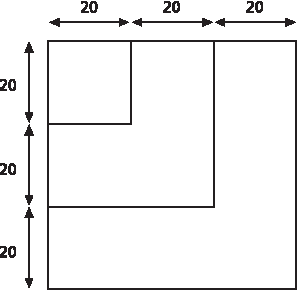
\includegraphics[width=6cm]{methods_logo}
			\caption{The company logo.}
			\label{fig:methods_logo}
		\end{figure}

	\section{Writing your own methods}
		Here, we will introduce the concept of creating our own methods. Initially, we will choose a toy example for simplicity, then move on to a more practical example.
		
		The Worldwide Cardboard Box Corporation has a logo, which consists of three squares within one another, as in \Vref{fig:methods_logo}.
		
		They wish to use this logo in several positions in a picture box, as in \Vref{fig:methods_logo_screen}. Here is the code to draw two identical logos at positions (10, 20) and (100, 100).
		\begin{lstlisting}
' Draw logo at top left
paper.DrawRectangle(myPen, 10, 20, 60, 60)
paper.DrawRectangle(myPen, 10, 20, 40, 40)
paper.DrawRectangle(myPen, 10, 20, 20, 20)
' Draw logo at bottom right
paper.DrawRectangle(myPen, 100, 100, 60, 60)
paper.DrawRectangle(myPen, 100, 100, 40, 40)
paper.DrawRectangle(myPen, 100, 100, 20, 20)
		\end{lstlisting}
		Note that the squares are of size 20, 40 and 60 pixels, with all their top left corners at the same point. Look at the code, and note that the three instructions to draw one logo are basically repeated, apart from the position of the top left of the logo. We will bundle up these three instructions as a method, so that a logo can be drawn with one instruction.

	\section{A first method}
		Here is a complete program, named Logo Method. It shows the creation and use of a method, which we chose to name \keyword{DrawLogo}. The VB style convention is to begin method names with a capital letter.
		\begin{lstlisting}
Private Sub Button1_Click(
	sender As System.Object,
	e As System.EventArgs) Handles Button1.Click
	Dim paper As Graphics
	paper = PictureBox1.CreateGraphics()
	Dim myPen As Pen = New Pen(Color.Black)
	DrawLogo(paper, myPen, 10, 20)
	DrawLogo(paper, myPen, 100, 100)
End Sub
Private Sub DrawLogo(drawingArea As Graphics,
	penToUse As Pen,
	xPos As Integer,
	yPos As Integer)
	drawingArea.DrawRectangle(penToUse, xPos, yPos, 60, 60)
	drawingArea.DrawRectangle(penToUse, xPos, yPos, 40, 40)
	drawingArea.DrawRectangle(penToUse, xPos, yPos, 20, 20)
End Sub
		\end{lstlisting}

		\begin{figure}[ht]
			\centering
			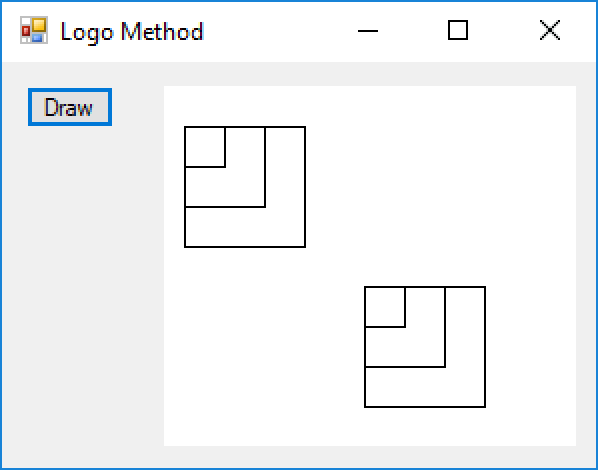
\includegraphics[width=6cm]{methods_logo_screen}
			\caption{Screenshot of the logo method program.}
			\label{fig:methods_logo_screen}
		\end{figure}


		The program has a picture box and a button. Clicking on the button causes two logos to be drawn, as in \Vref{fig:methods_logo_screen}.
		
		The concept of methods and arguments is a major skill that all programmers need to master. We will now discuss the program in detail. Look at the extract:
		\begin{lstlisting}
Private Sub DrawLogo(drawingArea As Graphics,
	penToUse As Pen,
	xPos As Integer,
	yPos As Integer)
		\end{lstlisting}
		This declares (introduces) the method, and is known as the method header. The word \keyword{Sub} is short for subroutine (another name for a method). The header states the name of the method (which we had the freedom to choose), and the items that must be supplied to control its operation. VB uses the terms \emph{arguments} and \emph{parameters} in this area - we shall examine them below. The rest of the method, ended by an \keyword{End Sub}, is known as the body, and is where the work gets done. Often the header is a long line, and we may choose to split it up at suitable points using space and underscore.
		
	\section{Calling a method}
		In VB, we call a private method by stating its name, together with a list of arguments in brackets. In our program, the first call is:
		\begin{lstlisting}
DrawLogo(paper, myPen, 10, 20)
		\end{lstlisting}
This statement has two effects:
		\begin{itemize}
			\item The argument values are automatically transferred into the method. We cover this in more detail below.
			\item The program jumps to the body of the method (the statements after the header), and executes the statements. When it runs out of statements and reaches the \keyword{End Sub}, execution is continued back at the point where the method was called from.
		\end{itemize}
The second call then takes place:
		\begin{lstlisting}
DrawLogo(paper, myPen, 100, 100)
		\end{lstlisting}
		\Vref{fig:methods_execution} illustrates this. There are two calls, producing two logos.

	\section{Passing arguments}
		It is essential to have an understanding of how arguments are transferred (i.e. passed) into methods. In our example, the concept is shown in the following lines:
		\begin{lstlisting}
DrawLogo(paper, myPen, 10, 20)
Private Sub DrawLogo(ByVal drawingArea As Graphics,
	ByVal penToUse As Pen, 
	ByVal xPos As Integer, 
	ByVal yPos As Integer)
		\end{lstlisting}
		The area to focus on is the two lists of items in brackets. In a call, the items are termed \emph{arguments}. In the header of the method, the items are termed \emph{parameters}. To clarify the situation, we will extract the parameters and arguments:
		\begin{center}
			\begin{tabular}{lllll}
				arguments: & \keyword{paper} &	\keyword{myPen} &	\keyword{10} &	\keyword{20}\\
				parameters:& \keyword{drawingArea}&	\keyword{penToUse} &	\keyword{xPos} &	\keyword{yPos}
			\end{tabular}
		\end{center}
		\begin{figure}[ht]
			\centering
			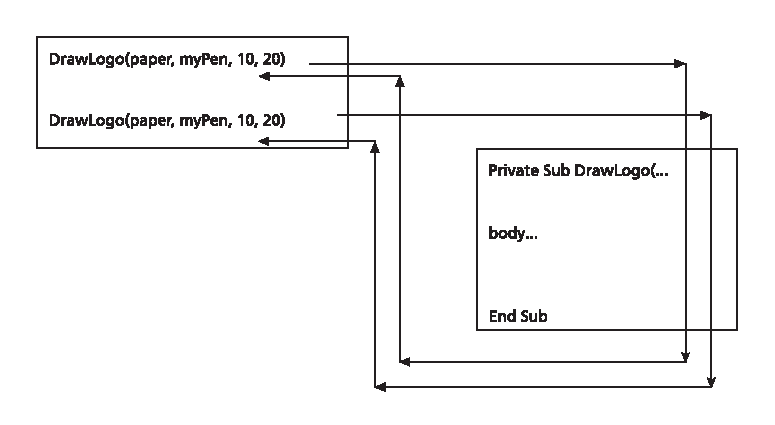
\includegraphics[width=11cm]{methods_execution}
			\caption{Execution path of two calls.}
			\label{fig:methods_execution}
		\end{figure}


		Recall our likening of a variable to a box. Inside the method, a set of empty boxes (the parameters) awaits the transfer of argument values. After the transfer, we have the situation shown in \Vref{fig:methods_args_param}. We don't have any numeric values to use for the passing of the drawing area and pen, so focus on the passing of the coordinates.
		
		The transfer takes place in a left-to-right order. The call must provide the correct number and type of arguments. If the caller (the user) accidentally gets arguments in the wrong order, the transfer process won't re-order them! When the \keyword{DrawLogo} method executes, the above values control the drawing process. Though we have called the method with numbers, we can use expressions (i.e. involving variables and calculations), as in:
		\begin{lstlisting}
Dim x As Integer = 6
DrawLogo(paper, myPen, 20 + 3, 3 * 2 + 1) ' 23 and 7
DrawLogo(paper, myPen, x * 4, 20) ' 24 and 20
		\end{lstlisting}
		\begin{figure}[ht]
			\centering
			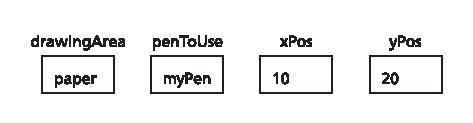
\includegraphics[width=8cm]{methods_args_param}
			\caption{Transferring arguments into parameters.}
			\label{fig:methods_args_param}
		\end{figure}

		In VB there are two ways to pass items to a method - by reference and by value. We cover passing by reference later in this chapter.

		\begin{stqb}
			\begin{STQ}
				\item	Whereabouts will the logos be drawn in the following code?
					\begin{lstlisting}
Dim a As Integer = 10
Dim b As Integer = 20
DrawLogo(paper, myPen, a, b)
DrawLogo(paper, myPen, b + a, b - a)
DrawLogo(paper, myPen, b + a - 3, b + a - 4)
					\end{lstlisting}
			\end{STQ}
		\end{stqb}

	\section{Parameters and arguments}
		There are two bracketed lists that we are discussing, and it is important to be clear about the purpose of each list:
		\begin{itemize}
			\item The writer of the method must choose which items the method will request via parameters. Thus, in \keyword{DrawLogo}, the dimensions of the nested squares are always set to 20, 40 and 60, so the caller need not supply this data. However, the caller might wish to vary the position of the logo, to use a different pen, or even to draw the logo on a different component (such as a button). These items have been made into parameters.
			\item The writer of the method must choose names for each parameter. If similar names are used in other methods, no problem arises - each method has its own copy of its parameters. In other words, the writer is free to choose any name.
			\item The writer of the method must choose how the argument will be passed into the parameter: the choice is between \keyword{ByVal} or \keyword{ByRef}. \keyword{ByVal} is implicitly chosen by default, as in all our introductory examples.
			\item The type of each parameter must be provided by using the \keyword{As} keyword, rather like its use in \keyword{Dim}. The types depend on the particular method. A comma is used to separate one parameter from another. Look at the \keyword{DrawLogo} header to see the arrangement.
			\item The caller must supply a list of arguments in brackets. The arguments must be in the correct order for the method, and must be of the correct type.
		\end{itemize}
The two benefits of using a method for the logo drawing are that we remove the
duplication of the three \keyword{DrawRectangle} statements when several logos are needed, and giving the task a name enables us to think at a higher level.
Finally, we recognize that you might wish to transfer the programming skills that you learn here into other languages. The concepts are similar, but the terminology is different: in many languages, the caller supplies 'actual parameters', and the method declaration has 'formal parameters'.

		\begin{stqb}
			\begin{STQ}
				\item	Explain what is wrong with these calls:
					\begin{lstlisting}
DrawLogo(paper, myPen, 50, "10")
DrawLogo(myPen, paper, 50, 10)
DrawLogo(paper, myPen, 10)
					\end{lstlisting}
				\item	Here is the call of a method:
					\begin{lstlisting}
JustDoIt("Oranges")
					\end{lstlisting}
					and here is the method itself:
					\begin{lstlisting}
Private Sub JustDoIt(fruit As String) 
  MessageBox.Show(fruit)
End Sub
					\end{lstlisting}
					What happens when the method is called?
			\end{STQ}
		\end{stqb}

	\section{A triangle method}
	In order to introduce more features of methods, we shall create a more useful method, which we shall name \keyword{DrawTriangle}. Because \emph{we} are writing the method (rather than making use of a pre-written one) we can choose what kind of triangle, and can choose the arguments that we want the caller to supply. We will choose to draw a right-angled triangle, pointing to the right, as in \Vref{fig:methods_triangle}.

		\begin{figure}[ht]
			\centering
			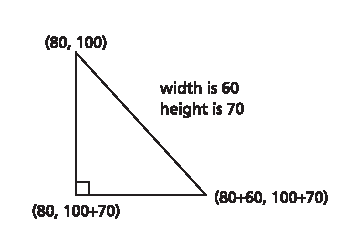
\includegraphics[width=6cm]{methods_triangle}
			\caption{Triangle coordinate calculations.}
			\label{fig:methods_triangle}
		\end{figure}
		
		In choosing arguments, there are a number of possibilities - for example we might demand that the caller gives us the coordinates of the three corners. However, we have chosen the arguments to be:
		\begin{itemize}
			\item the drawing area and pen, as before;
			\item the coordinates of the top point of the triangle;
			\item the width of the triangle;
			\item the height of the triangle.
		\end{itemize}
		Another way to regard these coordinates is that they specify the position of an enclosing rectangle for our right-angled triangle.
		
		We can draw the lines in any order. Let us examine the drawing process with numbers at first. As an example, we will draw a triangle with the top corner at (80, 100) and with a width of 60 and a height of 70. \Vref{fig:methods_triangle} shows the calculations. The process is:
		\begin{itemize}
			\item Draw from (80, 100) down to (80, 100+70). Remember that the \keyword{y} coordinate increases as we move down.
			\item Draw from (80, 100+70) across to (80+60, 100+70).
			\item Draw from the top corner (80, 100) diagonally to (80+60, 100+70).
		\end{itemize}
		Ensure that you can follow the above - maybe sketch it out on paper.
		
		Note that in our explanation, we did not simplify the calculations: we left 100+70 as it is, rather than as 170. When we come to the coding, the position of the triangle and the size of the triangle will be passed in as separate arguments.

		Here is a complete program which is named Triangle Method. It contains a \keyword{DrawTriangle} method. It also contains the \keyword{DrawLogo} method, to illustrate that a program can contain many methods.
		\begin{lstlisting}
Private Sub Button1_Click(
	sender As System.Object,
	e As System.EventArgs) Handles Button1.Click
	Dim paper As Graphics
	paper = PictureBox1.CreateGraphics()
	Dim myPen As Pen = New Pen(Color.Black)
	DrawLogo(paper, myPen, 10, 20)
	DrawLogo(paper, myPen, 100, 100)
	DrawTriangle(paper, myPen, 100, 10, 40, 40)
	DrawTriangle(paper, myPen, 10, 100, 20, 60)
End Sub
Private Sub DrawLogo(drawingArea As Graphics,
	penToUse As Pen,
	xPos As Integer,
	yPos As Integer)
	drawingArea.DrawRectangle(penToUse, xPos, yPos, 60, 60)
	drawingArea.DrawRectangle(penToUse, xPos, yPos, 40, 40)
	drawingArea.DrawRectangle(penToUse, xPos, yPos, 20, 20)
End Sub
Private Sub DrawTriangle(drawingArea As Graphics,
	penToUse As Pen,
	xPlace As Integer,
	yPlace As Integer,
	width As Integer, 
	height As Integer)
	drawingArea.DrawLine(penToUse, xPlace, yPlace,
		xPlace, yPlace + height)
	drawingArea.DrawLine(penToUse, xPlace,
		yPlace + height,
		xPlace + width, yPlace + height)
	drawingArea.DrawLine(penToUse, xPlace, yPlace,
		xPlace + width, yPlace + height)
End Sub
		\end{lstlisting}

		\begin{figure}[ht]
			\centering
			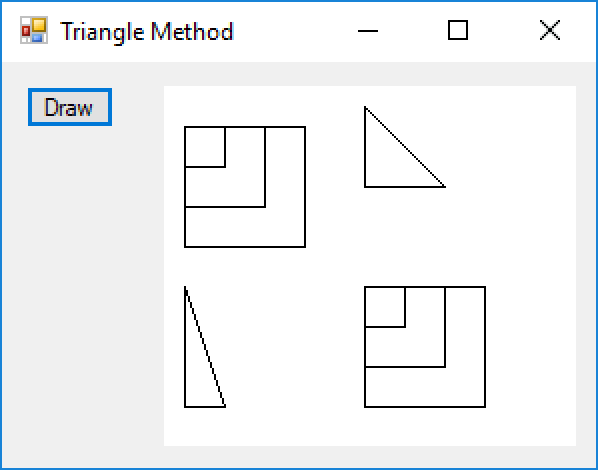
\includegraphics[width=6cm]{methods_triangle_screen}
			\caption{Triangle coordinate calculations.}
			\label{fig:methods_triangle_screen}
		\end{figure}

		It has a button and a picture box. Click on the button to draw two logos and two triangles. \Vref{fig:methods_triangle_screen} shows the output.
		Here are some points about the coding of the \keyword{DrawTriangle} method:
		\begin{itemize}
			\item We chose to name it \keyword{DrawTriangle}, but it is up to us. We could have chosen \keyword{Triangle}, or even \keyword{DrawThing}, but \keyword{DrawTriangle} fits with the names of the library methods.
			\item The names for the parameters: \keyword{drawingArea}, \keyword{penToUse}, \keyword{xPlace}, \keyword{yPlace}, \keyword{width}, and \keyword{height} were our choice.
			\item The order of the parameters was also under our control. We could re-code the method to require the height before the width if we wanted to. (We put the width first because many of VB's library methods use this order.)
		\end{itemize}
		So - we have our triangle. We will use it to look at local variables, and also show how it can be a 'building brick' for more powerful methods.

	\section{Local variables}
	In \Cref{ch:var}, we saw the use of \keyword{Dim} to declare variables, but we did not look at the relationship between variables and methods. Here we will do this.
		
		Look at this modified version of \keyword{DrawTriangle}, which we have named \keyword{DrawTriangle2}:
		\begin{lstlisting}
Private Sub DrawTriangle2(drawingArea As Graphics,
	penToUse As Pen,
	xPlace As Integer,
	yPlace As Integer,
  width As Integer,
	height As Integer)
	Dim rightCornerX, rightCornerY As Integer
	rightCornerX = xPlace + width
	rightCornerY = yPlace + height
	drawingArea.DrawLine(penToUse, xPlace, yPlace,
		xPlace, rightCornerY)
	drawingArea.DrawLine(penToUse, xPlace, rightCornerY,
		rightCornerX, rightCornerY)
	drawingArea.DrawLine(penToUse, xPlace, yPlace,
		rightCornerX, rightCornerY)
End Sub
		\end{lstlisting}
		It is called in just the same way as \keyword{DrawTriangle}, but internally it uses two variables, named \keyword{rightCornerX} and \keyword{rightCornerY}, which have been introduced to simplify the calculations. Look at how they are used to refer to the rightmost point of the triangle. These variables exist only within \keyword{DrawTriangle2}. They are local to the method (the terminology is that they have local \emph{scope}). If variables of the same name exist within other methods, then there is no conflict, in that each method uses its own copy. Another way to look at this is that when other programmers are creating methods they can invent local variables without cross-checking with everyone.

		The role of local variables is to assist in the work of the method, whatever it is doing. The variables have a limited scope, restricted to their own method. Their existence is temporary - they are created when a method is called, and destroyed when it exits.

		
	\section{Name clashes}
		In VB, the creator of a method is free to choose appropriate names for local variables and parameters - but what happens if names are chosen which clash with other variables? We could have:
		\begin{lstlisting}
Private Sub MethodOne(x As Integer,
	y As Integer)
	Dim z As Integer = 0
	' code ...
End Sub
Private Sub MethodTwo(z As Integer,
	x As Integer)
	Dim w As Integer = 1
	'code ...
End Sub
		\end{lstlisting}
		Let us assume that the methods have been written by two people. \keyword{MethodOne} has \keyword{x} and \keyword{y} as parameters, and declares an integer \keyword{z}. These three items are all local to \keyword{MethodOne}. In \keyword{MethodTwo}, the programmer exercises the right of freedom to name local items, and opts for \keyword{z},\keyword{x}, and \keyword{w}. The name clash of \keyword{x} (and of \keyword{z}) does not give a problem, as VB treats the \keyword{x} of \keyword{MethodOne} as different from the \keyword{x} of \keyword{MethodTwo}.

		\begin{stqb}
			\begin{STQ}
				\item	Here is the call of a method:
					\begin{lstlisting}
Dim a As Integer = 3
Dim b As Integer = 8
DoStuff(a, b)
MessageBox.Show(CStr(a))
					\end{lstlisting}
					and here is the method itself:
					\begin{lstlisting}
Private Sub DoStuff(x As Integer,
	y As Integer)
	Dim a As Integer = 0
	a = x + y
End Sub
					\end{lstlisting}
					What is shown in the message box?
			\end{STQ}
		\end{stqb}


		Let us summarize the method facilities we have discussed so far. Later we will include the \keyword{Return} statement, and the use of \keyword{ByRef}.
		\begin{itemize}
			\item The general form of a Sub declaration is:
				\begin{lstlisting}
Private Sub SomeName(parameter list)
	body 
End Sub
				\end{lstlisting}
				The programmer chooses the method name.
			\item The parameter list is a list of types and names, with the type of passing by default \keyword{ByVal}, if not specified. If a method does not need arguments, we use empty brackets for the parameter list when we declare it, and empty brackets for the argument list when we call it.
				\begin{lstlisting}
Private Sub MyMethod()
	body
End Sub
				\end{lstlisting}
	and the method call is:
				\begin{lstlisting}
MyMethod()
				\end{lstlisting}
			\item A class can contain any number of methods, in any order. In this chapter, our programs only consist of one class. The essence of the layout is:
				\begin{lstlisting}
Public Class Form1
	Private Sub SomeName(parameter list ...)
		body
	End Sub
	Private Sub AnotherName(parameter list ...)
		body
	End Sub
End Class
				\end{lstlisting}
				We will make use of the \keyword{Class} and \keyword{End Class} keywords in \Vref{ch:classes}. For now, merely note that a class can group together a series of methods.
		\end{itemize}

		
	\section{Event-handling methods}
		A class contains a set of methods. We write some of them ourselves (such as \keyword{DrawLogo}) and we explicitly call them. However there are other methods which VB creates for us, such as:
		\begin{lstlisting}
Private Sub Button1_Click
		\end{lstlisting}
		When is this method called? The answer is that the VB system routes all events (such as button-clicks, mouse-clicks, etc.) to their appropriate event method, provided that a matching method exists. Normally, we never call these methods ourselves.


	\section{Function methods and results}
		In our previous examples of arguments and parameters, values were passed \emph{into} methods, which the method made use of. However, often we need to code methods which perform a calculation and send a result back to the rest of the program, so that the result can be used in subsequent calculations. In this case we must use a \keyword{Function} method, rather than a \keyword{Sub} method. Let us look at a function method which calculates the area of a rectangle, given its two sides as input arguments. Here is the complete program, named Area Function:
		\begin{lstlisting}
Private Sub Button1_Click(sender As System.Object,
	e As System.EventArgs) Handles Button1.Click
	Dim a As Integer
	a = AreaRectangle(10, 20)
End Sub
Private Function AreaRectangle(
	length As Integer,
	width As Integer) As Integer
	Dim area As Integer
	area = length * width
	Return area
End Function
		\end{lstlisting}
		There are a number of new features in this example, which go hand in hand.
		
		Examine the function header:
		\begin{lstlisting}
Private Function AreaRectangle(
	length As Integer,
	width As Integer) As Integer
		\end{lstlisting}

		Instead of \keyword{Sub}, we have used \keyword{Function}. Also, we need to specify the type of item that the function will return to the caller. In this case, because we are multiplying two \keyword{Integer} values, the type of the answer will also be an \keyword{Integer}. The final \keyword{As Integer} in the function header states that \keyword{AreaRectangle} will return an \keyword{Integer} to us.

		The choice of this type depends on the problem. For example, it might be an integer or a string, but it could also be a more complicated object such as a picture box or button. The writer of the function chooses what type of value is returned.
		
		To return a value from the function, we make use of the \keyword{Return} statement. We put:
		\begin{lstlisting}
Return expression
		\end{lstlisting}
		The expression (as usual) could be a number, a variable or a calculation (or even a function call), but it must be of the correct type, as specified in the declaration of the method - i.e. its header. Additionally, the \keyword{Return} statement causes the current method to stop executing, and returns immediately to where it left off in the calling method. Now we will look at how a function can be called.
		
		Here is how \emph{not} to call a function. They cannot be used as complete statements, as in:
		\begin{lstlisting}
AreaRectangle(10, 20)    'wrong
		\end{lstlisting}
		Instead, the caller must arrange to 'consume' the returned value. Here is an approach to understanding the returning of values: imagine that the method call (the name and argument list) is erased, and is replaced by the returned result. If the resulting code makes sense, then VB will allow you to make such a call. Look at this example:
		\begin{lstlisting}
answer = AreaRectangle(30, 40)
		\end{lstlisting}
		The result is 1200, which we imagine as replacing the call, effectively giving:
		\begin{lstlisting}
answer = 1200
		\end{lstlisting}
		This is valid VB. But if we put:
		\begin{lstlisting}
AreaRectangle(30, 40)
		\end{lstlisting}
		the substitution would produce a VB statement consisting only of a number:
		\begin{lstlisting}
1200
		\end{lstlisting}
		which is meaningless. Here are some more ways that we might consume the result:
		\begin{lstlisting}
Private Sub Button2_Click(sender As System.Object,
												e As System.EventArgs) Handles Button2.Click
	Dim n As Integer
	n = AreaRectangle(10, 20)
	MessageBox.Show("area is " & CStr(AreaRectangle(3, 4)))
	n = AreaRectangle(10, 20) * AreaRectangle(7, 8)
End Sub
		\end{lstlisting}

		\begin{stqb}
			\begin{STQ}
				\item	Work through the above statements with pencil and paper, substituting results for calls.
			\end{STQ}
		\end{stqb}
		To complete the discussion of \keyword{Return}, note that it can be used with \keyword{Sub} methods. In this case, we must use \keyword{Return} without specifying a result, as in:
		\begin{lstlisting}
Private Sub Demo(ByVal n As Integer)
	' do something
	Return
	' do something else
End Sub
		\end{lstlisting}
		This can be used when we want the method to terminate at a statement other than the last one.
		
		Let us look at an alternative way of coding our area example:
		\begin{lstlisting}
Private Function AreaRectangle2(length As Integer,
	width As Integer)
	As Integer
	Return length * width
End Function
		\end{lstlisting}
		Because we can use \keyword{Return} with expressions, we have omitted the variable \keyword{area} in \keyword{AreaRectangle2}.

		Such reductions in program size are not always beneficial, because the reduction in meaningful names can reduce clarity, hence leading to more debugging and testing time.

		\begin{stqb}
			\begin{STQ}
				\item	Here is a function named Twice, which returns the doubled value of its \keyword{Integer} argument.
					\begin{lstlisting}
Private Function Twice(ByVal n As Integer) As Integer
	Return 2 * n
End Function
	Here are some calls:
Dim n As Integer = 3
Dim r As Integer
r = Twice(n)
r = Twice(n + 1)
r = Twice(n) + 1
r = Twice(3 + 2 * n)
r = Twice(Twice(n))
r = Twice(Twice(n + 1))
r = Twice(Twice(n) + 1)
r = Twice(Twice(Twice(n)))
					\end{lstlisting}
					For each call, state the returned value.
			\end{STQ}
		\end{stqb}

		
	\section{Building on methods}
	As an example of methods which make use of other methods, let us create a method which draws a primitive 'lean-to' house with a cross-section shown in \Vref{fig:methods_house}. 
		
		The height of the roof is the same as the height of the walls, and the width of the wall is the same as the width of the roof. We will choose the \keyword{Integer} arguments 
to be:
		\begin{itemize}
			\item the horizontal position of the top right point of the roof;
			\item the vertical position of the top right point of the roof;
			\item the height of the roof (excluding the wall);
			\item the width of the house. The triangle for the roof and the rectangle for the walls have the same width.
		\end{itemize}
		We will use \keyword{DrawRectangle} from the VB library, and use our own \keyword{DrawTriangle}.

		\begin{figure}[ht]
			\centering
			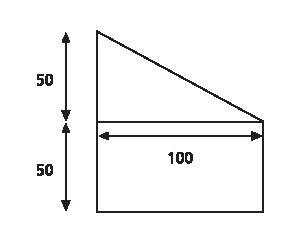
\includegraphics[width=6cm]{methods_house}
			\caption{House with width of 100 and roof height of 50.}
			\label{fig:methods_house}
		\end{figure}

		\begin{figure}[ht]
			\centering
			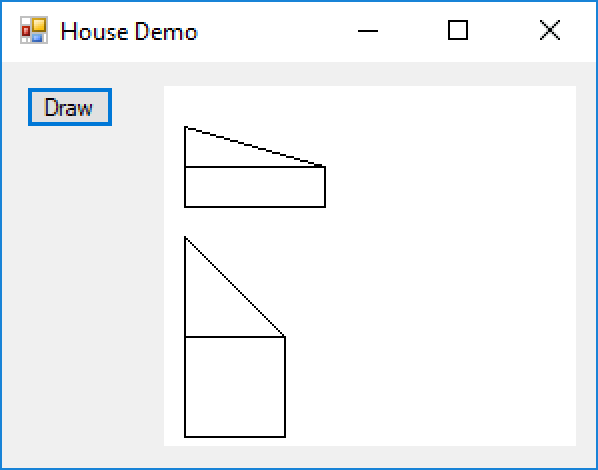
\includegraphics[width=6cm]{methods_house_screen}
			\caption{Screenshot of house demo program.}
			\label{fig:methods_house_screen}
		\end{figure}

		
		Here is the program, with the resulting images shown in \Vref{fig:methods_house_screen}.
		\begin{lstlisting}
Private Sub Button1_Click(
	sender As System.Object,
	e As System.EventArgs) Handles Button1.Click
	Dim paper As Graphics
	paper = PictureBox1.CreateGraphics
	Dim myPen As Pen = New Pen(Color.Black)
	DrawHouse(paper, myPen, 10, 20, 70, 20)
	DrawHouse(paper, myPen, 10, 90, 50, 50)
End Sub
Private Sub DrawHouse(ByVal drawingArea As Graphics,
	penToUse As Pen,
	topRoofX As Integer,
	topRoofY As Integer,
	width As Integer,
	height As Integer)
	DrawTriangle(drawingArea, penToUse, topRoofX,
		topRoofY, width, height)
	drawingArea.DrawRectangle(penToUse, topRoofX,
		topRoofY + height, width, height)
End Sub
Private Sub DrawTriangle(drawingArea As Graphics,
	penToUse As Pen,
	xPlace As Integer,
	yPlace As Integer,
	width As Integer,
	height As Integer)
	drawingArea.DrawLine(penToUse, xPlace, yPlace,
		xPlace, yPlace + height)
	drawingArea.DrawLine(penToUse, xPlace,
		yPlace + height,
		xPlace + width, yPlace + height)
	drawingArea.DrawLine(penToUse, xPlace, yPlace,
		xPlace + width, yPlace + height)
End Sub
		\end{lstlisting}
		The program is straightforward if you recall that:
		\begin{itemize}
			\item Methods return to where they were called from, so:
				\begin{itemize}
					\item \keyword{Button1\_Click} calls \keyword{DrawHouse};
					\item \keyword{DrawHouse} calls \keyword{DrawRectangle};
					\item \keyword{DrawHouse} calls \keyword{DrawTriangle};
					\item \keyword{DrawTriangle} calls \keyword{DrawLine} (three times).
				\end{itemize}
			\item Arguments can be expressions, so \keyword{yPlace + height} is evaluated, then passed into \keyword{DrawLine}.
			\item The \keyword{width} and \keyword{height} of \keyword{DrawHouse} and the \keyword{width} and \keyword{height} of \keyword{DrawTriangle} are totally separate. Their values are stored in different places.
		\end{itemize}
		You will see that what might have been a longer program has been written as a short program, split into methods with meaningful names. This illustrates the power of using methods.


	\section{Passing arguments by reference}
		So far, we have used the concept of passing arguments by value, either with a sub or a function. We use a function when a single value needs passing back to the caller. This seems fine initially, but there is another situation not yet covered - what if our method needs to pass back more than one result? Here is such a situation:
		\begin{quote}
			Given a number of cents, write a method to calculate the equivalent whole number of Euros, and the number of cents remaining. We have one input and two results.
		\end{quote}
		Before we look at the VB approach to returning several results, we need to look more deeply into the nature of passing arguments. Previously, we stated that we pass \emph{values} of arguments. This seems obvious - what else could we do? In fact, VB also allows us to pass arguments \emph{by reference} as well as by value and we can use this facility to pass back any number of results from a method.
		
		Here is an analogy to illustrate passing by reference: imagine that you are working on a written report, with some friends. Your friend asks you for the report. There are two ways you could pass this document to them:
		\begin{itemize}
			\item You could photocopy the document.
			\item You could tell your colleague 'Oh yes that one. Just look on the fourth shelf down. There it is'.
		\end{itemize}
		The analogy:
		\begin{itemize}
			\item The document is an argument.
			\item Your colleague is a method who is being called by you, to whom an argument is to be passed.
			\item Passing a photocopy of the document is passing 'by value'.
			\item Telling your colleague where the original copy is stored at is termed 'passing by reference'.
		\end{itemize}
		There are two important points about these ways of passing arguments:
		\begin{itemize}
			\item Passing a copy of the data (by value) is safer. You keep hold of the original item. Any changes your colleague makes will \emph{not} affect your copy.
			\item Passing the whereabouts of the data (passing by reference) is fast. In fact, no data is physically moved, and your colleague can make changes without removing the document from your room. But remember that there is only a single copy of the item. Your colleague has the same power as you have to change this single copy. Sometimes you will want this, but sometimes you won't.
		\end{itemize}
		Bearing in mind the concepts of passing by value and passing by reference, let us look at how your computer's random access memory (RAM) is organized. The precise organization is rather complicated but, approximately, RAM consists of millions of storage boxes, known as memory locations. Each location has an address, rather like numbered houses on a street. Each variable we create is stored at a particular place in memory. In other words, each variable is associated with an address.
		
		Now we reach the point about passing by reference: if we wish to pass a variable to a method, there are two choices:
		\begin{itemize}
			\item Either we pass a copy of the current value.
			\item Or we pass the address. In VB jargon we pass a reference to the variable. When the method knows the whereabouts of a variable, it knows which memory location to look in. In other languages, a reference is known as a \emph{pointer}.
		\end{itemize}

		\begin{stqb}
			\begin{STQ}
				\item	Imagine that we have a large number of variables stored in RAM. If we know the value of a variable, is it possible to find out where the variable is stored?
			\end{STQ}
		\end{stqb}
		Let us move closer to VB. The way we can obtain \emph{several} results from a method is as follows:

		Before calling a method, the caller declares some variables, to be regarded as places for holding results calculated by the method. When the method is called, the addresses of the variables (the references) are passed into the method. The method can make use of the original values of the variables if it needs to, and it can also assign new values to them.
		
		Though this sounds rather complicated, the manipulation of references is done behind the scenes in VB, as we will see.


	\section{References - an example}
	Let us tackle the problem posed earlier: a method which converts a number of cents into a whole number of dollars, and the cents left over. This will involve coding a method which has one input and two results. \Vref{fig:var_eurocents} shows a screenshot of the Euros Method program, and here is the code, which uses a text box to obtain the number of cents, and labels to display the results. We used a similar GUI in \Vref{ch:var}, when we did this task without using a function.
		\begin{lstlisting}
Private Sub Button1_Click(sender As System.Object,
		e As System.EventArgs) Handles Button1.Click
	Dim originalCents, wholeEuros, centsLeft As Integer
	originalCents = CInt(TextBox1.Text)
	EurosAndCents(originalCents, wholeEuros, centsLeft)
	EurosLabel.Text = CStr(wholeEuros)
	CentsLabel.Text = CStr(centsLeft)
End Sub
Private Sub EurosAndCents(totalCents As Integer,
			ByRef euros As Integer,
			ByRef centsLeft As Integer)
	euros = totalCents \ 100
	centsLeft = totalCents Mod 100
End Sub
		\end{lstlisting}
		The property settings are as follows:
		\begin{center}
			\begin{tabular}{lll}
				\toprule Control &	Property	 & Setting \\ \midrule
				Button1 & Text & Calculate\\
				TextBox1 & Text & (empty)\\
				EurosLabel & Text & (empty)\\
				CentsLabel & Text & (empty) \\ \bottomrule
			\end{tabular}
		\end{center}

		Here are some points about the above program:
		\begin{itemize}
			\item We chose the name \keyword{EurosAndCents} for the method.
			\item The method has two results, so we could not use the \keyword{Return} statement.
			\item We use \keyword{ByRef} to pass references.
			\item The \keyword{totalCents} parameter is passed by value, as it is the default by omission, or explicitly by prefixing the parameter with \keyword{ByVal}. We \emph{could} have passed it by reference, but the method does not place a new value in this variable. Passing by value ensures that the method cannot change the original value, hence is safer.
			\item \keyword{euros} and \keyword{centsLeft} are passed by reference. In effect, they are empty boxes and we are informing \keyword{EurosAndCents} of their whereabouts.
			\item When the method assigns a new value to \keyword{centsRemaining}, it is actually using the variable \keyword{centsLeft}, declared in \keyword{Button1\_Click}. In other words, \keyword{centsRemaining} stands for \keyword{centsLeft}.
			\item As usual, the writer of a method has free choice of argument names. In this example, one name was the same as the caller chose (\keyword{euros}) and the other pairs were different (\keyword{originalCents}, \keyword{cents}, and \keyword{centsLeft}, \keyword{centsRemaining}). Perhaps \keyword{Euros} was used twice because the same person both wrote the method and called it. For large programs, this will not be the case, and in general, the names differ.
		\end{itemize}


		\begin{stqb}*
			\begin{STQ}
				\item	Would \keyword{EurosAndCents} work correctly if we re-coded it as:
					\begin{lstlisting}
Private Sub EurosAndCents2(a As Integer,
		ByRef b As Integer,
		ByRef c As Integer)
	b = a \ 100
	c = a Mod 100
End Sub
					\end{lstlisting}
				\item 	Here is the call of a method:
					\begin{lstlisting}
Dim x As Integer = 4
Dim y As Integer = 9
DoWork(x, y)
					\end{lstlisting}
					and here is the method:
					\begin{lstlisting}
Private Sub DoWork(a As Integer,
		ByRef b As Integer)
	a = a + 1
	b = b + 1
End Sub
					\end{lstlisting}
					What are the resulting values of \keyword{x} and \keyword{y}?
			\end{STQ}
		\end{stqb}

	\section{References: a \keyword{Swap} method}
		A classic example of the use of arguments is to code a method which swaps over the values of two variables. First, here is the code without making use of a method:
		\begin{lstlisting}
aCopy = a
a = b
b = aCopy
		\end{lstlisting}
		Note that if we put:
		\begin{lstlisting}
a = b
b = a
		\end{lstlisting}
		then both \keyword{a} and \keyword{b} end up set to the original value of \keyword{b}.
		
		So, rather than some code which only works for the variables \keyword{a} and \keyword{b}, we want to bundle the code up as a method which works for any names. There are two arguments, and the method changes their value. Here is the code:
		\begin{lstlisting}
Private Sub Swap(ByRef a As Integer, ByRef b As Integer)
	Dim aCopy As Integer
	aCopy = a
	a = b
	b = aCopy
End Sub
		\end{lstlisting}
		Note that the method needs the references of the variables and their values. But we don't need to pass four arguments, because once a method has the reference, it can also use the value. Here are some examples of calling the \keyword{Swap} method:
		\begin{lstlisting}
Dim a As Integer = 6
Dim b As Integer = 8
Dim c As Integer = 20
Dim d As Integer = 30
Swap(c, d)
Swap(a, b)
Swap(a, c)
		\end{lstlisting}
		Here are some incorrect calls of \keyword{Swap}:
		\begin{lstlisting}
Dim a As Integer = 3
Swap(a, 6)
		\end{lstlisting}
		
		In VB, numbers (and the results of calculations) have a value, but \emph{not} a reference. In other words, they are not stored at a known place in RAM. So, when supplying arguments, we \emph{must} use variable names where \keyword{ByRef} has been used. In the above example, because 6 does not have a reference, there is no place to accept the value of \keyword{a}. The program will compile and run, but the only effect of the method is to set \keyword{a} to 6. However, where a method stipulates implicit or explicit \keyword{ByVal}, we can supply a variable \emph{or} a calculation.


	\section{\keyword{Me} and objects}
		You are probably reading this book because VB is an object-oriented language, but you might be wondering why this chapter has not mentioned objects. The truth is that methods and objects are vitally connected. When you run small VB programs, you are running an instance of a class, i.e. an object. This object contains methods (e.g. \keyword{Swap}) and properties (which we have not yet covered).

		When an object calls a method which is declared within itself, we can simply put
		\begin{lstlisting}
Swap(a, b)
		\end{lstlisting}
		or we can use the full object notation, as in
		\begin{lstlisting}
Me.Swap(a, b)
		\end{lstlisting}
		\keyword{Me} is a VB keyword, and stands for the currently running object. So you have been doing object-oriented programming without realizing it. Here are some examples:
		\begin{lstlisting}
Swap(a, b)
'works as above
Me.Swap(a, b)
'compilation error
Me.DrawLine(myPen, 10, 10, 100, 50)
		\end{lstlisting}
		In the above, an error is detected because we are asking VB to locate the \keyword{DrawLine} method within the current object. In fact, \keyword{DrawLine} exists outside the program in the \keyword{Graphics} class, and must be called in this way:
		\begin{lstlisting}
Dim paper As Graphics
paper = PictureBox1.CreateGraphics()
paper.DrawLine(myPen, 10, 10, 100, 50)
		\end{lstlisting}


	\section{Overloading}
		Our \keyword{Swap} method is useful, in the sense that it can work on arguments with any name. The drawback is that they must be integers. Recall the code:
		\begin{lstlisting}
Private Sub Swap(ByRef a As Integer, ByRef b As Integer)
	Dim aCopy As Integer
	aCopy = a
	a = b
	b = aCopy
End Sub
		\end{lstlisting}
		But what if we wanted to swap two \keyword{Double} variables? We will code \emph{another} \keyword{Swap} method, intentionally coding it differently:
		\begin{lstlisting}
Private Sub Swap2(ByRef a As Double, ByRef b As Double)
	Dim aCopy As Double
	aCopy = a
	a = b
	b = aCopy
End Sub
		\end{lstlisting}
		However, it would be convenient to use the same name for both methods, and in VB we can. Here is how we code the method declarations:
		\begin{lstlisting}
Private Sub Swap(ByRef a As Integer, ByRef b As Integer)
	Dim aCopy As Integer
	aCopy = a
	a = b
	b = aCopy
End Sub
Private Sub Swap(ByRef a As Double, ByRef b As Double)
	Dim aSafe As Double = a
	Dim bSafe As Double = b
	a = bSafe
	b = aSafe
End Sub
		\end{lstlisting}

		Now we call the methods:
		\begin{lstlisting}
Dim c As Integer = 3
Dim d As Integer = 4
Dim g As Double = 1.2
Dim h As Double = 4.5
Swap(c, d)
Swap(g, h)
		\end{lstlisting}
		How does VB decide which method to use? There are two methods named \keyword{Swap}, so VB additionally looks at the number of parameters and at their types. In our example, if \keyword{a} and \keyword{b} had been declared as \keyword{Double} variables, VB would call the method which swaps doubles. The code contained by the methods can be different - it is the number of parameters and their types that determine which method is called.
		
		If the method is a function, the return type plays no part in overloading, i.e. it is the parameter types of the function which must be different.
		
		What we have done is termed \emph{overloading}. The \keyword{Swap} method has been overloaded with several possibilities.
		
		So if you are writing methods which perform similar tasks, but differ in the number of arguments and/or types, it is sensible make use of overloading by choosing the \emph{same} name rather than invent an artificially different name.
		
		There are hundreds of examples of overloading used in the VB libraries. For example, there are four versions of \keyword{DrawLine}.


	\section{Passing objects to methods}
		In our examples we have concentrated on passing numbers, but we also need to pass more complicated objects, such as pens and picture boxes. Here is an example, in which we pass two numbers to be added, and also pass the label where the result is to be displayed:
		\begin{lstlisting}
Private Sub ShowSum(display As Label,
	a As Integer, b as Integer)
	display.Text = CStr(a + b)
End Sub
		\end{lstlisting}
		Here is how we might call the method:
		\begin{lstlisting}
ShowSum(Label1, 3, 4)
ShowSum(Label2, 5, 456)
		\end{lstlisting}
		Passing an object by value allows us to manipulate its properties and call its methods.

	\section{Programming principles}
		\begin{itemize}
			\item A method is a section of code which has a name. We call the method by using its name.
			\item We can use subroutine methods and function methods.
			\item We can pass arguments to a method. They can be passed by value or by reference.
			\item Passing by value is the safer of the two approaches. Passing by reference allows the method to change the original item.
			\item When a method returns only one value, use a function.
			\item If you can identify a well-defined task in your code, consider separating it out and writing it as a method.
		\end{itemize}


	\section{Programming pitfalls}
	\begin{itemize}
		\item The method header must include type names. The following is wrong:
			\begin{lstlisting}
Private Sub MethodOne(x)   ' wrong
			\end{lstlisting}
			Instead we must put, for example:
			\begin{lstlisting}
Private Sub MethodOne(x As Integer)
			\end{lstlisting}
		\item A method call must not include type names. For example, rather than:
			\begin{lstlisting}
MethodOne(y As Integer)
			\end{lstlisting}
	we put:
			\begin{lstlisting}
MethodOne(y)
			\end{lstlisting}
		\item When calling a method, you must supply the correct number of arguments and the correct types of arguments.
		\item You must arrange to consume the result of a function in some way. The following style of call does not consume a return value:
			\begin{lstlisting}
SomeFunction(e, f)
			\end{lstlisting}
		\end{itemize}


	\section{Grammar spot}
		\begin{itemize}
			\item The general pattern for methods takes two forms. First, for a \keyword{Sub} method (that does not return a result), we declare the method by:
				\begin{lstlisting}
Private Sub MethodName(parameter list)
	body
End Sub
				\end{lstlisting}
				and we call the method by a statement, as in:
				\begin{lstlisting}
MethodName(argument list)
				\end{lstlisting}
			\item For a \keyword{Function} method, the form is:
				\begin{lstlisting}
Private Function FunctionName(parameter list) As some type
	body
End Function
				\end{lstlisting}
				Any type or class can be specified as the returned type.
			\item We call the function as part of an expression, e.g.:
				\begin{lstlisting}
n = FunctionName(a, b)
				\end{lstlisting}
			\item The body of the function method must include a \keyword{Return} statement featuring the correct type of value.
			\item When a method has no arguments, we use empty brackets (  ) in both the declaration and the call.
			\item The parameter list is created by the writer of the method. If a parameter is not prefixed, it is by default \keyword{ByVal}, otherwise \keyword{ByRef} has to be used, a name, and a type.
			\item The argument list is written by the caller of the method. It consists of a series of items in the correct (matching) order, and of the correct types. Unlike parameters within a method, the type names are not used.
		\end{itemize}

		
	\section{New language elements}
		\begin{itemize}
			\item The declaration of private \keyword{Sub} and \keyword{Function} methods.
			\item The call of a method, consisting of the method name and arguments.
			\item The use of \keyword{Return} to simultaneously exit and pass a value back from a function method.
			\item The use of \keyword{Return} to exit from a \keyword{Sub} method.
			\item The use of overloading.
			\item The use of \keyword{Me} to stand for the current object.
		\end{itemize}


	\section{New IDE facilities}
		There are no new IDE facilities introduced in this chapter.


	\section{Summary}
		\begin{itemize}
			\item Methods contain subtasks of a program.
			\item We can pass arguments into methods.
			\item Using a method is termed \emph{calling} the method.
			\item Function methods return a result.
		\end{itemize}

	\section{Exercises}
		To try out the methods you write, build a simple GUI with text boxes, labels and message boxes, as required. Use a button click to execute your code.
		The first problems involve \keyword{Sub} methods, and passing by value:

		\begin{EXE}
			\item Write a method named \keyword{ShowName}, with one String parameter. It should display the supplied name in a message box.
			\item Write a method named \keyword{ShowNames}, with two string parameters representing your first name and your last name. It should display your first name in a message box, and then display your last name in another message box.
			\item Write a method named \keyword{DisplayEarnings}, with two integer parameters representing an employee's salary, and the number of years they have worked. 
The method should display their total earnings in a message box, assuming that 
they earned the same amount every year.
			\item Code a method which draws a circle, given the coordinates of the centre and the radius. Its header should be:
				\begin{lstlisting}
Private Sub Circle(	drawingArea As Graphics,
		penToUse As Pen, xCentre As Integer,
		yCentre As Integer, radius As Integer)
				\end{lstlisting}
			\item \label{it:drawstreet} Code a method named \keyword{DrawStreet}, which draws a street of houses, using the provided \keyword{DrawHouse} method. For the purposes of this question, a street consists of four houses, and there should be a 20-pixel gap between each house. The arguments provide the location and size of the leftmost house, and are identical to \keyword{DrawHouse}.
			\item Code a method (to be known as \keyword{DrawStreetInPerspective}), which has the same arguments as Exercise \ref{it:drawstreet}. However, each house is to be 20 per cent smaller than the house to its left.
		\end{EXE}

		The following programs involve function methods with arguments passed by value:
		\begin{EXE}
			\item Write a function method which returns the inch equivalent of its centimetre argument. An example call is:
				\begin{lstlisting}
Dim inches As Integer = InchEquivalent(10.5)
				\end{lstlisting}
				Multiply centimetres by 0.394 to calculate inches.
			\item Write a method which returns the volume of a cube, given the length of one side. A sample call is:
				\begin{lstlisting}
Dim vol As Double = CubeVolume(1.2)
				\end{lstlisting}
			\item Write a method which returns the area of a circle, given its radius as an argument. A sample call is:
				\begin{lstlisting}
Dim a As Double = AreaCircle(1.25)
				\end{lstlisting}
				The area of a circle is given by the formula 
				\begin{lstlisting}
Math.PI * r * r
				\end{lstlisting}
				Though we could use a number such as 3.14, a more accurate value is provided by \keyword{Math.PI}.
			\item \label{it:SecsIn} Write a function method named \keyword{SecsIn}, which accepts three integers, representing a time in hours, minutes, and seconds. It should return the total time in seconds. A sample call is:
				\begin{lstlisting}
Dim totalSecs As Integer = SecsIn(1, 1, 2) 'returns 3662
				\end{lstlisting}
			\item Write a function method which returns the area of a solid cylinder. Decide one of its parameters. You should call \keyword{AreaCircle} from above, to assist in calculating the area of the top and bottom. The circumference of a circle is given by
				\begin{lstlisting}
2 * Math.PI * r
				\end{lstlisting}
			\item Write a function method called \keyword{Increment}, which adds 1 to its integer argument. An example of a call is:
				\begin{lstlisting}
Dim n As Integer = 3
Dim a As Integer = Increment(n)    'returns 4
				\end{lstlisting}
		\end{EXE}

		The following problems involve \keyword{Sub} and \keyword{Function} methods, and passing arguments by reference and value:
		\begin{EXE}
			\item Write a sub method named \keyword{SumAndDifference}, which calculates the sum and the difference of any two integer values (i.e. if the input arguments are 3 and n, it passes back 3+n, and 3-n.)
			\item Write a sub method named \keyword{SecsToHMS}, which takes in a number of seconds, and converts it into hours, minutes and seconds. Make use of the \keyword{Mod} and \ operators. (For example, 3662 seconds is 1 hour, 1 minute, and 2 seconds.)
			\item \label{it:Input3} Write a sub method named \keyword{Input3}, which has three integer arguments, passed by reference. It should use three input boxes to input three integers from the user. Here is how we might call it:
				\begin{lstlisting}
Dim a, b, c As Integer
Input3(a, b, c)
				\end{lstlisting}
			\item Write a function method named \keyword{TimeDifferenceInSecs}, with six arguments passed by value and an integer result. It takes in two times, in hours, minutes and seconds, and returns the difference between them in seconds. Use the \keyword{Input3} method from Exercise \ref{it:Input3}, and \keyword{SecsIn} from Exercise \ref{it:SecsIn}.
			\item Write a sub method named \keyword{HMSBetween}, which accepts two times in seconds, and passes back the hours, minutes and seconds between them. Your method should make use of \keyword{SecsToHMS}.
			\item \label{it:Increment} Write a sub method named \keyword{Increment}, which increments its integer argument. An example of a call is:
				\begin{lstlisting}
Dim v as Integer = 4
Increment(v)    'v is now 5
				\end{lstlisting}
		\end{EXE}

		The following problems involve overloading:
		\begin{EXE}
			\item Use any program which contains \keyword{SecsIn}. Add an additional function method also named \keyword{SecsIn}, which has two arguments, for minutes and seconds.
			\item Use your program from Exercise \ref{it:Increment}, with \keyword{Increment} in use. Write two other versions of \keyword{Increment}: one with a \keyword{Double} argument, and one with a \keyword{String} argument. The latter should use the \keyword{\&} operator to join a space on to the end of the string.
		\end{EXE}


		\begin{stab}
			\begin{enumChapter}
				\item	At (10, 20), (30, 10), (27, 26).
				\item In the first call, the quotes should not be used. They indicate a string, not an integer.

						In the second call, the paper and the pen are in the wrong order.

						In the third call, an argument is missing
				\item A message box displaying \keyword{Oranges} will appear.
				\item The message box displays the original value of \keyword{a}, which is 3. The \keyword{a} that is set to 11 inside the method is a local variable.
				\item Here are the stages in replacing a call by its result. For
					\begin{lstlisting}
n = AreaRectangle(10, 20)
					\end{lstlisting}
					we have:
					\begin{lstlisting}
n = 200
					\end{lstlisting}
					For the line
					\begin{lstlisting}
MessageBox.Show("area is " & CStr(AreaRectangle(3, 4)))
					\end{lstlisting}
					we have the stages:
					\begin{lstlisting}
MessageBox.Show("area is " & CStr(12))
MessageBox.Show("area is 12")
					\end{lstlisting}
					For the line
					\begin{lstlisting}
n = AreaRectangle(10, 20) * AreaRectangle(7, 8)
					\end{lstlisting}
					we have the stages:
					\begin{lstlisting}
n = 200 * 56
n = 11200
					\end{lstlisting}

				\item The values that r takes are:
					\begin{lstlisting}
6
8
7
18
12
16
14
24
					\end{lstlisting}
				\item No. Several variables might hold the same value, so values are not unique. To use a house number analogy: houses have an address and a value (e.g. the number of people currently in a house). We could not track down the address of the house containing three people, because there are many such houses.
				\item It would work correctly - though the names are not very meaningful. The writer of a method has free choice of parameter names; they need not match names used by the caller of the method. It is, however, the responsibility of the caller to supply arguments in the correct left-to-right order.
				\item	The value of \keyword{x} is left at 4, and the value of \keyword{y} changes to 10. Within the method, changing \keyword{a} to 5 only has a local effect. Passing by value prevents the original variable \keyword{x} from being altered.
			\end{enumChapter}
		\end{stab}



